\documentclass[12pt]{article}
% \pagestyle{empty}

\usepackage{fullpage}
%\usepackage{cyrillic}
\usepackage{url}
\usepackage[usenames]{color}
\usepackage{amssymb}
\usepackage{graphicx}
\usepackage{amscd}
\usepackage{amsmath}
\usepackage{hyperref}
\usepackage{graphicx}

\graphicspath{ {images/} }
\usepackage[colorlinks=true,
linkcolor=webgreen,
filecolor=webbrown,
citecolor=webgreen]{hyperref}

\definecolor{webgreen}{rgb}{0,.5,0}
\definecolor{webbrown}{rgb}{.6,0,0}


\usepackage[parfill]{parskip}

\thispagestyle{empty}

\begin{document}
\begin{titlepage}
	\centering
	\vspace{4cm}
	{\scshape\Large Game Development\par}
	\vspace{6.5cm}
	{\huge\bfseries Guide to Unity 101\par}
	\vspace{2cm}
	{\Large\itshape Benjamin Zhao\par}
	\vfill
	Artwork courtesy of\par
	{\itshape Calvin ``Ippers'' Ip\par}
  \vfill
	In preperation for\par
	Global Game Jam 2017\par
	\vspace{2cm}
	
% Bottom of the page
	{\large \today\par}
\end{titlepage}

\newpage
\section{Introduction}

This guide is a software development approach to game development using Unity 5.4.1. 

The following sections will run you through a series of exercies to pick up Unity's 2D game development tools for the upcoming Global Game Jam. In this guide, we will learn the basic tools of the Unity software, understand how to interact with and between the Unity engine, and integrate your visual assets into game animations. Once you have finished these exercises, you should not only be able to apply the techniques learned here but also be able to explore new content and Unity features as a pioneer for your next indie game. 

Before you begin, make sure you have Unity 5.4.1+ installed and ready to be run on your computer. Open it up and create a new blank project. Congratulations, you have created your first game! (Cheesy line but you need to feel good about getting started). 

\section{Understanding Unity}

Check out the introduction to Unity2D here: \url{https://unity3d.com/learn/tutorials/topics/2d-game-creation/introduction-unity-2d-perspective}

Watch the 45 minute video (we all know its ``long and tedious''). Of course you're not going to get everything in one go, but there are some key points that only professional game developers can give that this guide can't!

Unity is a game engine in which you can build your game foundations on. Unity provides various tools and libraries accessible using the Unity studio that you can use to help build the interactions in your game. Let's quickly go over some of the main tabs and functions you'll need to start developing.

\subsection{Hierarchy} 

The hierarchy tab located on the center left holds data about all game objects that currently exist in the scene (a scene is a game instance aka level). Notice that just like in OOP, the heirarchy also displays the child parent relationships between objects. Quite commonly, these parent-child relationships refer to relative transform, rotation and scaling. Imagine designing a character who holds a sword and a shield. We say that the sword and shield are children of the player. If the player moves, both objects move. If the player drops the sword, perhaps we take the sword object out of the player and break the parent-child relationship. The sword is now a standalone object in the hierarchy (eg attaching the camera to the character is a great way to make a following camera).

\subsection{Scene/Game}
The scene/game tabs are located in the center of the studio. These are your graphical tools which help visualize the current state of the game. You can easily manipulate objects in the scene tab, and test the current progress of your game in the game tab. Make sure to use the play and pause button to test your game!

\subsection{Inspector}
Located on the center right is the inspecter tab. Any object that you click in the hierarchy shows a set of properties on the inspecter tab. These properties define the game object. This includes transform, sprite renderers, physics bodies, colliders, effectors and your own scripts! You start here as a developer.

\subsection{Project}
Located at the bottom half of the screen is the project tab. This tab manages your file hierarchy of your project. Drag and drop assets and create your scripts here or check out your Unity project folder in your computer's respective file explorer and look for the Assets folder. This is where all your assets (sprites, animations, scripts, scenes, prefabs) are located. Soon enough you'll find the game to explode with a couple thousand scripts, a million sprites and a whole bunch of other nonsense. Later this guide will show you a sample directory hierarchy to properly organize your files (it's going to get messy fast)!

\subsection{Other tools that you'll need later}
Just for fun, if you want to know more about Unity's tools, here's a list for you to Google up (you'll definitely be using them later so don't skimp out cause you're lazy)! \\
1. Console - You should already know why\\
2. Sprite Editor - Helps you cut your image into sprites\\
3. Animation - Your go to window to help piece together an animation from a set of sprites\\
4. Animator - A visual blueprint that maps your animations together based on conditions\\
5. Monodevelop - Your IDE for C\#/Javascript/Boo (you can change this)\\

\newpage

\subsection{Let's Get Started! - Get your project Github Ready}
Here's a little exercise before we start the next section. Remember that new project you just created? Let's make that Github ready. What you need to know is that in your Unity project, there's a lot of auto generated metadata and libraries that do not need to be pushed onto your repo. 

Follow this guide here to setup your Unity project to Github ready: \url{http://stackoverflow.com/questions/21573405/how-to-prepare-a-unity-project-for-git}

The .gitignore is optional from the link, but you should use one (Github also provides a default Unity gitignore). Add your current project to Github, and you're ready to make progress!

\newpage

\section{Sweating the Small Stuff - Objects and Properties}

In this section we will go over how to create objects in Unity and attach properties to that object to allow for interaction. 

Start by right clicking your hierarchy window and create an sprite 2D object. You'll notice that the object already has the transform and sprite renderer properties (components) attached to it. The transform component is attached to all game objects. This specifies the position, rotation and scaling of the object. You can play around with the numbers on the component, or visually drag your object in the scene window and see how the component interacts. Sprite renderer displays a sprite on the game window. Take the image Char3-0.png and put it in your assets folder. Try to update the sprite renderer component with this image (so we can actually see your object). 

\subsection{Enter Physics}

Unity provides their own physics engine and object interactions. Let see if we can utilize them. Enter components Rigidbody2D and Box Collider2D. Take a look at the Unity documentation: \url{https://docs.unity3d.com/Manual/index.html}.

Let's try a simple exercise. Take that object from above and lets name it ``Player'' or something (just to give it an alias). Try adding the Rigidbody2D component to the player object. What happens? Try turning on and off isKinematic (and figure out what that means). 

Hint: Your character may fall to oblivion. Actually your character doesn't ever go away so make sure all your objects are to destroy themselves when you get rid of them!

Well this is boring. Lets add a platform for our character to stand on. Just create a new sprite 2D object, attach any sprite and change the x and y scalings to match some ground-like look. Make sure to add a box collider2D to the ground and lets try it out!
\\\\
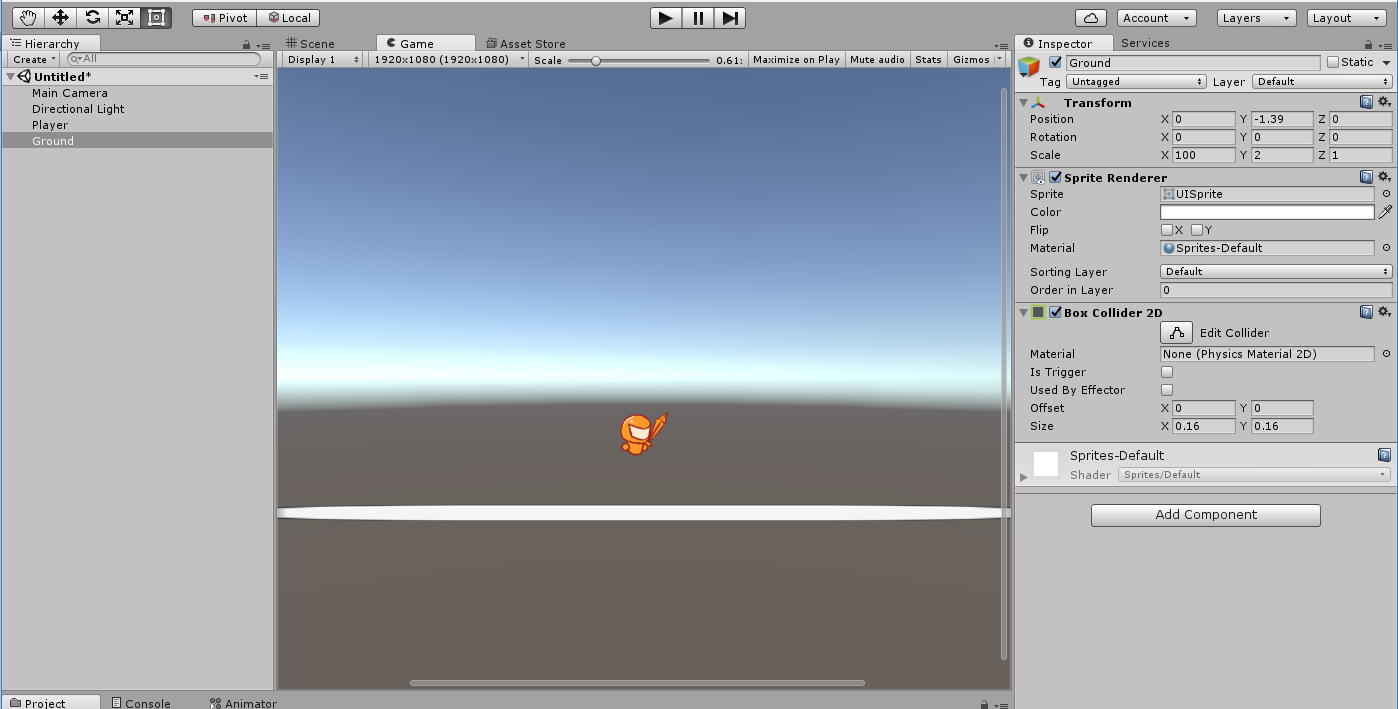
\includegraphics[scale=0.5]{Figure0311}

Ok well maybe it didn't work out quite as expected! Did you want the character to stand on the ground instead of falling through it? Well if you figured out the solution even before testing it then props to you! Worry not if you tested the code without thinking, you just aren't paying enough attention! No worries, I won't tell you how to fix it. You figure it out yourself!

Hint: Ghosts can't collide with colliders!

Let's break down what we've done. Rigidbody2D are like attaching physics properties to an object. They are objects that are affected by force, and torque. Rigid bodies however aren't directly affected by collisions (you can't hit Gengar with a Body Slam anyways) and we'll need to add a collider2D to our object if we want it to exhibit collisions with other colliders. 

Genius thought: Have you tried spawning your player at the corner end of our ground and try falling? Your character actually rotates because falling on a vertex may exhibit a small torque on your player. How would you freeze the rotation of said character? (Think about which axis is actually rotating)!

\newpage

\subsection{Movement - Our First Script}

Before we dive into actually writing our script that moves our character, let's talk about the many ways we can move our character, and the physics behind each movement. To do this, we'll need to go over the human anatomy (just kidding)!

Recall Newtonian physics 101 (I'm going to assume you've been introduced to this before), and Newton's laws. For more info, checkout: \url{http://hyperphysics.phy-astr.gsu.edu/hbase/Newt.html}\\
1. Newton's First Law states that an object will remain at rest or in uniform motion in a straight line unless acted upon by an external force. (Inertia)\\
2. Newton's Second Law is force, $F = ma$ \\
3. Newton's Third Law states that all forces have an equivalent but opposite reaction.

How does newtonian laws of motion help us understand how to move our character? Think to yourself the different types of motion that our player can exhibit before continuing to read. 

\begin{center}
    \begin{tabular}{| l | p{10cm} | }
    \hline
    Movement & Summary \\ \hline
    Position & We can update our player's location directly based on position. Here we exhibit the idea of ``teleportation''. \\ \hline
    Velocity & We can change the velocity of our player's Rigidbody2D to move in the direction we want. We can also do rocket physics (conservation of momentum)!\\ \hline
    Force & We can't directly modify a character's acceleration value (I think) but we can apply a force onto a single point on our object. Use newton's 2nd and 3rd laws to help you figure out what the force needed to create the target acceleration is.\\ \hline
    \end{tabular}
\end{center}
\vspace{1.5cm}

Sweet! Now you can make an educated choice on how to move your player! For this guide, we'll focus simply modifying our player's velocity with a custom script. Add a new custom C\# script component to your player (call it whatever you want related to movement). Monodevelop will open and we'll work on the script from there.

If you are working on C\#, you'll notice that the class extends MonoBehaviour, which a bunch of predefined functions (eg Start, Update). Just assume that MonoBehaviour is your class of function to object references Unity provides for you. You'll also note the Unity libraries that are auto imported. We actually just need to focus on writing the Start and Update functions. The start function is called when the object has finished being instantiated. The update function is called every frame.

\newpage

Here's a quick exercise: Write up the functions needed to change the velocity of the character left and right. You should start by grabbing a reference to the object's Rigidbody2D in the Start function (check out the GetComponent$<$T$>$() documentation). In the update function, you should continually check for input (check out the Input documentation) and update the velocity according to the button pressed. For more details check out: \url{http://answers.unity3d.com/questions/667641/how-do-i-move-my-2d-object-using-arrow-keys-also-h.html}

Extra: If you used Input.GetKey(), try using Input.GetAxis() instead. The reason why GetKey isn't preferred is because GetAxis controls can be mapped through Unity settings so you aren't limited to only the key you chose to begin with.

Extra: Another Monobehaviour function is known as fixedUpdate. Since update is called per frame, frame rate likely affects your game. To avoid this, you can/should use fixedUpdate to change in-game transforms, and velocity. Update can accurately pick up user input however so use them together. Here's some more info about fixedUpdate vs update: \url{http://answers.unity3d.com/questions/10993/whats-the-difference-between-update-and-fixedupdat.html}

Extra: Let's at least make our character look left and right when he moves. We can simply change the transform scale of the object by flipping it on the y axis. (In case you need another hint, try multiplying the scale by -1).

Genius thought: Why don't I change the velocity only when there is an input? Isn't it more computationally efficient? Yes but remember that inertia might have side effects on your character if you aren't careful! You want your character to stop when you let go of the input, otherwise by Newton's first law your character will maintain the velocity unless otherwise acted upon.

\subsection{A Little More on Scripting}

It may seem very troublesome to modify the velocity of your character through your script everytime you wanted to try out different values. Fear not, Unity's inspectors tab lets you modify the value through the UI instead of doing it through your script. How does Unity know what variables you can modify? In your script's class, make variables public and they'll appear on the UI!

How does this make Unity scripting even more powerful? Not only can primitive types (eg int, char) be passed through the UI, we can also pass references to other objects! Here's a good example of when you might want to have objects references. Suppose you made a game where your player owns a pet. How can we make sure the pet follows the player? We can write a script for the pet that moves to wherever the player moves. Our pet script would then need to hold a reference to our player, which we define as: \begin{verbatim} public GameObject player \end{verbatim}
And then drag and drop the referenced player through the UI onto the inspector. Here we can easily change the reference of the pet. For example an antagonist bribes the pet with cookies and follows the enemy instead (we change that with another script!).

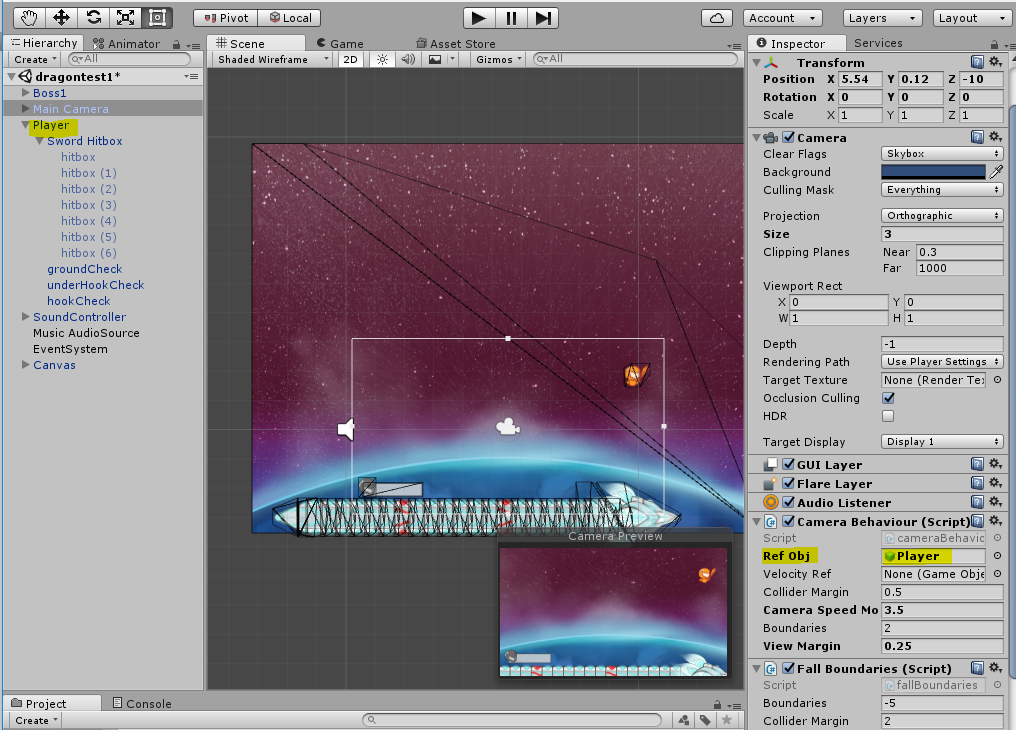
\includegraphics[scale=0.6]{Figure0331}
\\\\
Notice that our main camera object has a reference to our player. This is a custom script controlling the movement of the camera based according to the location of the player.

\subsection{Prefabs}

Well now that you feel content with your player object, you want to apply the same player to every level (kind of like in Super Mario Bros) where your character starts out the same at the beginning of every stage. Well isn't it a hassle to reconstruct your character at every scene? Or perhaps you want to randomly spawn meteors dropping from the sky; do you really want to write code to generate the entire meteor object then spawn it?

Prefabs are a way to save your resuable objects. Simply drag your object from the hierarchy tab and drop it into the project tab in any folder you see fit. A prefab will hold the object's hierarchy, components and default values (this doesn't apply to object references) and you can simply re-use the prefab by dragging the prefab object from the project tab back to the hierarchy. You can also invoke the prefab instance through a script to spawn the object during runtime (such as a meteor shower).

Design objects and scripts to be re-useable as much as possible. It'll make your game much more scalable. The hardest part is always getting the first level done. Once that's over its just a matter of making more stages (I could be wrong).    

\newpage

\section{The Life of the Party - Animations}

Remember back in chapter 3 when we briefly mentioned the sprite renderer component. A sprite renderer displays a static sprite during runtime. This is great for static objects like a background, but not our player (unless it was intended). 

There are many ways to create animations, but this guide will only serve the purpose of using sprites instead of models. A sprite is essentially a picture. We can generate animations from a set of sprites by changing the sprite every x number of frames (inversely proportional to how smooth the game is). By choosing from a set of animations, we can give life to our character; walking, jumping, sleeping - the sky is the limit on this one.

\subsection{Cutting Up the Sprite Sheet}

An animation should be a loop-able set of sprites that we'll iterate through within a number of frames. The more frames it takes to go through one cycle, the slower the animation will be. We group these sprite sets based on the action a character is performing. We want to make animations for all actions our character can perform. Let's first see how we should handle a sprite sheet.

A sprite sheet contains a sets of sprites grouped together. Some sprite sheets are grouped so that they can be cut into pixel grids, with each grid being of the same size. Other sprite sheets however take a little more work, requiring a referencial pivot for each sprite. When developing with your artist, make sure to communicate how the sprite sheets should be cut out. \\\\
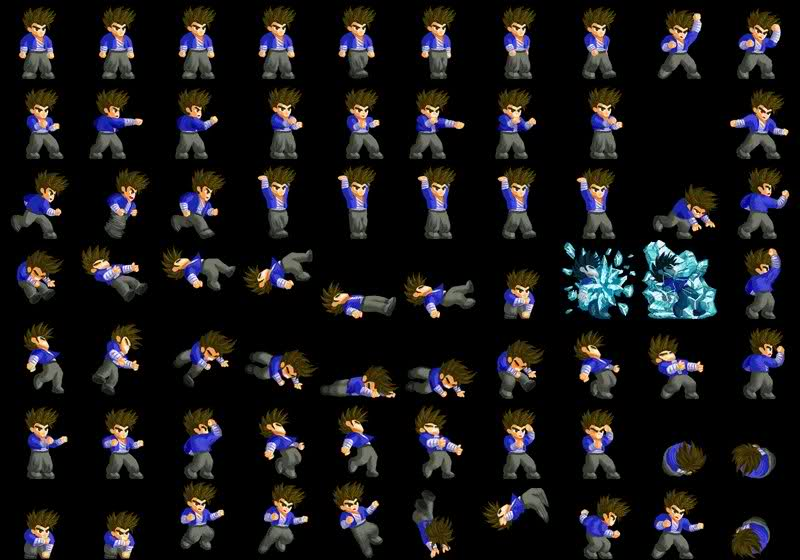
\includegraphics[scale=0.35]{Figure0411} \\

Here is an old favourite from Little Fighter 2. Notice that each sprite in the sprite sheet is held with a grid of the same size. This makes cutting the sprite sheet very easy.

Take the image CharacterSpritesheet4-1.png and copy it to your project folder. By clicking it on your Unity project tab, you'll be shown in the inspecter tab how to deal with the image. Let us set the right import settings. Change the type to Sprite (2D and UI), and the sprite mode to Multiple (if it's on single it'll assume the image is one sprite). Keep all others on default (check out the other settings on your own free time). Click on the Sprite Editor on the inspector and you'll be taken to the sprite editor window. In the top left, you'll find the slice menu, and based on your rules set with your artist, cut the sprite sheet accordingly. In this case, we'll use slice grid by cell size 150 X 150. \\\\
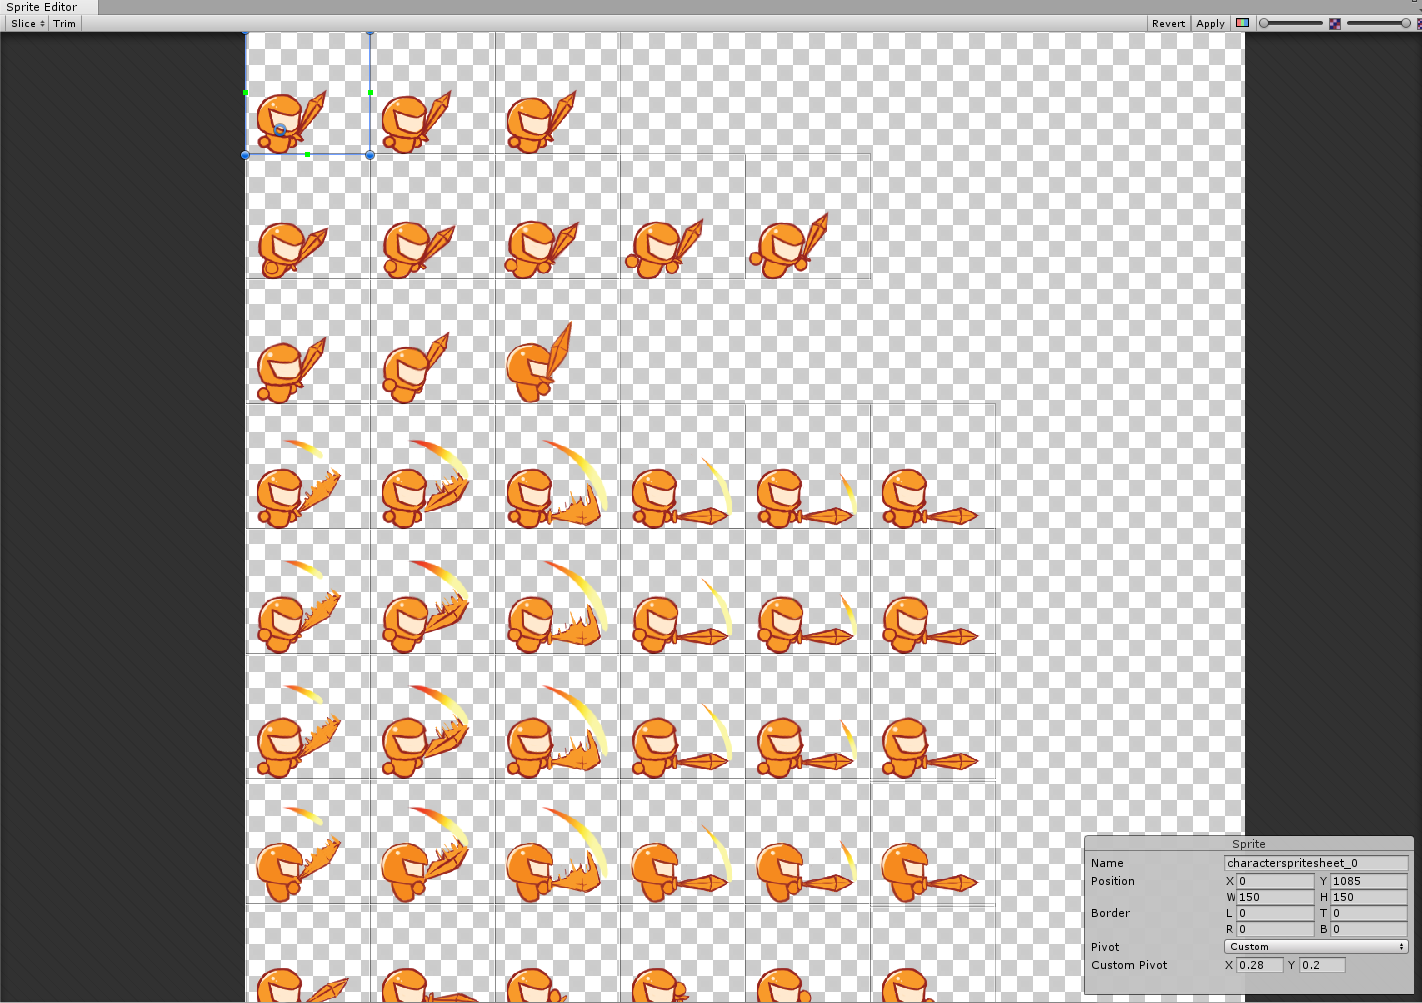
\includegraphics[scale=0.4]{Figure0412} \\

You'll have something similar to this image once you have done all that. Make sure to apply your changes! Go back to the project tab, you'll now see a small arrow beside the spritesheet, and if you expand it you'll see all the sprites that have been cut. You're now ready to make your first animation!

Extra: You'll notice a pivot setting defaulted to center when you were in your sprite editor. The pivot setting refers to the center of the object located on your sprite. It's not necessary, but you can move the pivot just between the head and the body of your sprite, and make that the custom pivot location for each cut.

\subsection{Making the Animation}

Let us jump right into making the animation. An animation as we've mentioned before should be a loop-able set of sprites that pertain to one action. In this case let's try to animate the idle animation (the first row of sprites). 

Open up the animation tab under window, and you'll need to click the object you want to animate. Click on your player, and create a new animation, call it idle. The animation window helps us iterate through a set of sprites given the frames per second (by default this is 60). Try dragging the first sprite from our cut spritesheet onto the animation window at time 0:00. Then drag the following second, third and second sprites to 0:01, 0:02 and 0:03 respectively. Try clicking the play button on the animation and watch your scene view. Perhaps the animation was too fast? Try playing around with the frame rate until you've found a liking to your animation.

You'll notice that your player object now has an animator component attached to it. This is the animation tree that does the animation management for the object. We'll discuss more about this in the next chapter. For now, test run your game and watch your character come to life!

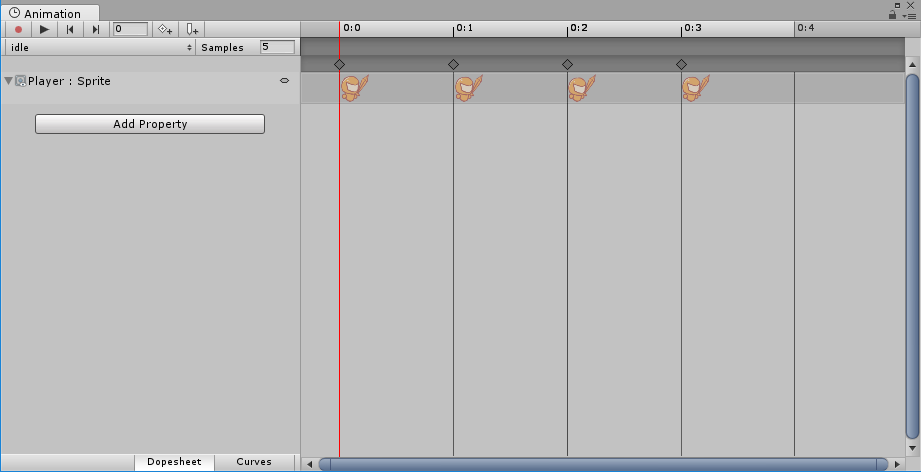
\includegraphics[scale=0.6]{Figure0421} \\

Genius thought: Can we put multiple sprites in an animation? The answer is yes we can! We can not only animate sprites by changing them, we can change the entire object over time! A parent object may not only animate itself, it can also change the transforms and animations of its children objects. With this idea, we can animate pieces seperately creating jointed effects.  

\subsection{The Animation Tree}

Recall the animator component on your player. You'll notice a controller already attached to the component. Unity automatically generates an animation tree when you've built your first animation. Let's see what it looks like so far. Go to window and open up the animator. 

Unity animator has three default states: Entry, Any State, and Exit. You'll also notice your idle state is attached from the Entry state. Therefore on game start, the animation transitions from Entry to Idle. 

Imagine Unity's animation tree to be like finite state machines (from computational theory). A state transitions to another state if all transition conditions are met. In this case, Unity provides a nice visual UI of how to build and maintain all of this. A state defines the animation it will be running. A transition defines the exit time (how long we'll run the state for) and a set of primitive variables (float, bool, trigger) that if met, will transition to the next state. We'll need to write an animation script in order to handle the transition variables.

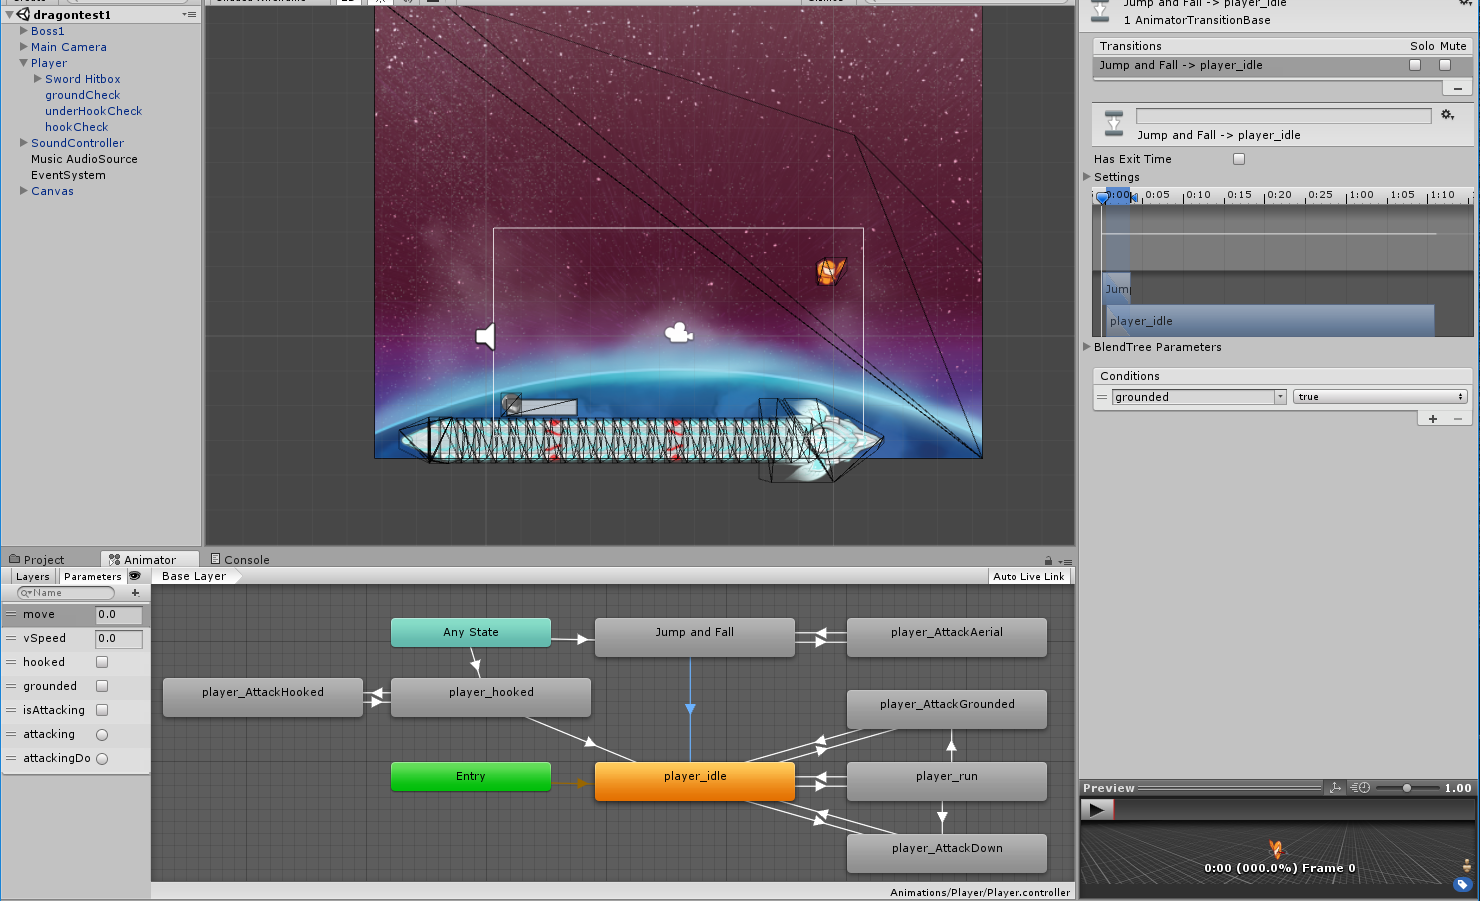
\includegraphics[scale=0.4]{Figure0431} \\

For practice, lets try to animate between idling when the character is standing, and running when the character is moving. We'll first start by creating the transition variables and the animation script, which is just a set of helper functions which if called, modifies the transition variables on the animation tree. Then we will go back to our movement script, and call these helper functions from animation script to modify the transition variables during runtime, and then we'll build our animation tree to transition between idle and running.

You'll notice in the animator tab, there is a subsection on the left called parameters. Here is where you'll define the parameters for your animation tree. Let's create a new float called speed (this is going to be the magnitude of the velocity). Now lets create a new script called playerAnims (note these names are all arbitrary) and attach that script to our player. It will use GetComponent$<$Animator$>$() to grab the animator component. The animator has the function that we'll need: setFloat(String variableName, float value), and we'll write a static helper function to modify that value. Check out the documentation of the animator for more details: \url{https://docs.unity3d.com/ScriptReference/Animator.html}    

Now back in our player controller script, we'll need to call the helper function defined in playerAnims at every update (or fixedUpdate if that is what you are using to move your player) to keep our animator speed value updated by passing in the velocity.magnitude.

Lastly, lets visually script the running animation. First we'll need to actually create the animation (refer back to section 4.2). Now that your running animation is created, it should appear on your animation tree, but not linked to anything. Let's create a transition from the idle to the running animation. We can do this by right clicking idle, and select make transition and click on the running state. Now click on the actual transition itself, and add a new condition based on speed (say speed $> 0.1$). We'll need to make a transition back from running state to idle state so we do the reverse (make sure your condition is speed $\leq 0.1$). 

Now lets try running your game. You should see your character switch between animations when moving! Is there delay between switching transitions? We can fine tune the delay by going back to the transitions, and changing the time settings. Try unchecking the setting Has Exit Time. Play around with these values until you've found a nice balance. 

Genius thought: Remember when we added our flipping function back in section 3.2 (to make our character look left and right)? We'll this is the fruit our our labour back when we didn't even have animations. Instead of needing to animation both left and right versions, we can flip the animations of facing right, and project the facing left version saving a huge amount of time and effort!


\subsection{The Melee Effect - Animation Cancelling}
Animation cancelling can be a difficult problem to fix with your game if you aren't careful. This happens when events cause the player to prematurely end their animation and possible ending lag as well. Frame cancelling is a form of animation cancelling in which a character skill's number of frames of execution is cut short. This becomes a notable problem in many competitive and hitbox dependent games. In our platformer game, we could've easily introduced frame cancelling techniques such as attacking in mid-air. In order for our game to continually feel smooth and refined, our player would likely need to cut short the attacking animation when landing. Short hopping aerials allows our player to dish out the most damage while being particularly safe doing so. I refer to this problem as the melee effect, based off of Super Smash Bros Melee.

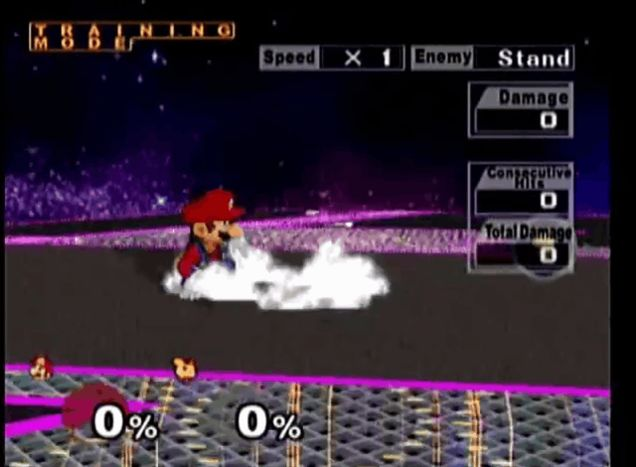
\includegraphics[scale=0.4]{Figure0441} \\

Super Smash Bros Melee is a prime example of where animation cancelling skills have drastically changed the way the game is played. Wavedash is one of the most commonly known exploitation of animation cancelling (perhaps in a good way). Wavedashing uses the momentum from air dodging but without the adverse effects of frame locking yourself to the air dodging mechanic. 

League of Legends have similar animation cancelling problems that exist in the game. Auto attack cancelling is a form of animation cancelling where a player deals damage in the middle of an auto attack but cancels the ending lag by performing an auto attack resetter commonly found on certain skills and items.

It's incredibly difficult to avoid these problems and each one is game specific. Some of the best advice from here is to plan out your animation tree far ahead of time, and identify as many animation cancelling problems that adversely affect the difficultly of your game as possible. When designing your animation-hitbox pairs, try to make hitboxes come later (but not too late) if a move is cancel-able. Add extra scripts if necessary to punish cancelled animations such as putting in extra ending lag (but by doing so makes our player less responsive). If unavoidable, then try to adjust the animation so that cancelling would only provide little to no benefits at all during practical gameplay.

\newpage

\section{Good Luck - Have Fun}
Thanks for going through this guide. Hopefully it'll have served the purpose as a good start toward designing your dream game. Build on your skills by play games, and making games. The possibilities are endless. Focus on making games that you can finish.

Remember, the best feeling of making games is when people enjoy the games you make. Also test your work! You don't want to get one of these: \\\\
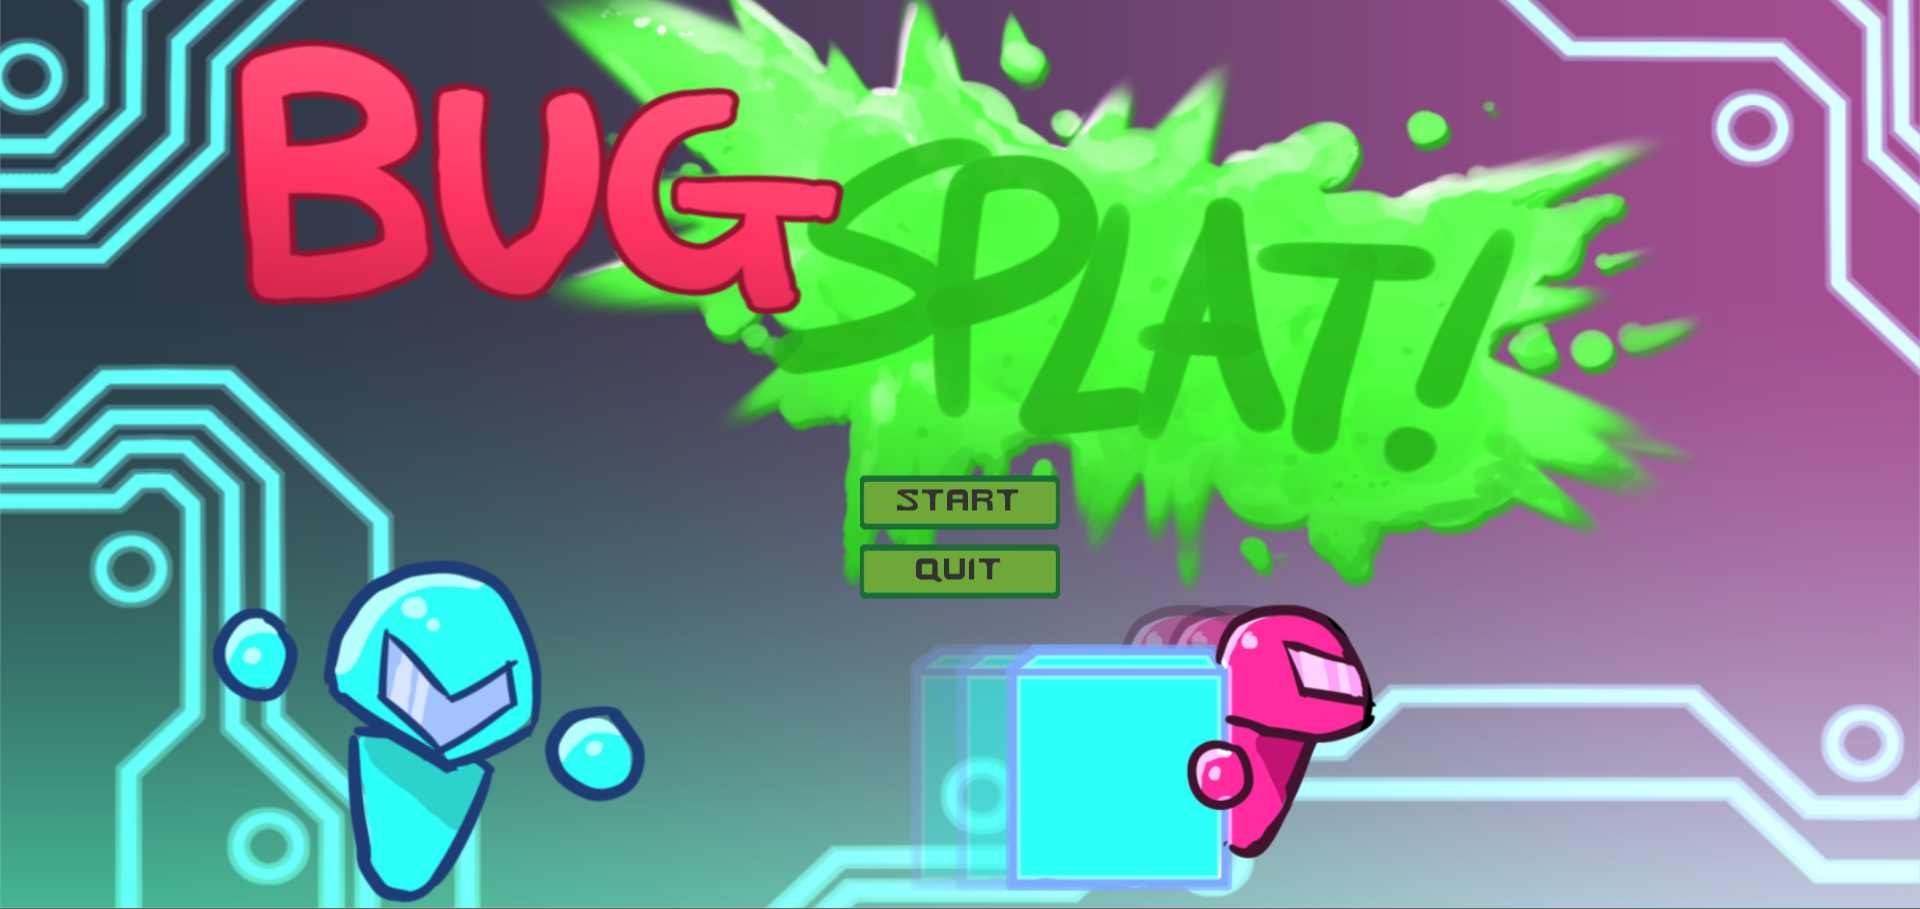
\includegraphics[scale=0.3]{Figure0501}


\end{document}
